\documentclass[english]{SPFShortReport}
\usepackage{subfigure}
\usepackage{spfFigures}
\usepackage{longtable}
\usepackage{url}
\usepackage{gensymb}
\usepackage[yyyymmdd,hhmmss]{datetime}
\reportName{Python calculation for heat pump SIN-75TU}
\reportSubName{Parametric Heat Pump calculation} 
\reportDate{\today \hspace{0.1cm} at: \currenttime \hspace{0.1cm} h} 
\author{Dani Carbonell}
\address{dani.carbonell@solarenergy.ch}
\begin{document}
\begin{table}[!ht]
\begin{small}
\caption{Fitted coefficients for the heat pump.}
\begin{center}
\resizebox{12cm}{!} 
{
\begin{tabular}{l | c c } 
\hline
\hline
Coefficient &Description & \\ 
 & &$[kW]$\\ 
\hline
$PQ_{1}$ & \emph{$1^{st}$ condenser polynomial coefficient}  & 7.0114e+01    \\ 
$PQ_{2}$ & \emph{$2^{st}$ condenser polynomial coefficient}  & 7.6974e+02    \\ 
$PQ_{3}$ & \emph{$3^{st}$ condenser polynomial coefficient}  & 1.9787e+02    \\ 
$PQ_{4}$ & \emph{$4^{st}$ condenser polynomial coefficient}  & -1.2662e+03    \\ 
$PQ_{5}$ & \emph{$5^{st}$ condenser polynomial coefficient}  & 1.0354e+03    \\ 
$PQ_{6}$ & \emph{$6^{st}$ condenser polynomial coefficient}  & -1.0177e+03    \\ 
\hline
$PCOP_{1}$ & \emph{$1^{st}$ COP polynomial coefficient}  & 6.3036e+00    \\ 
$PCOP_{2}$ & \emph{$2^{st}$ COP polynomial coefficient}  & 4.6365e+01    \\ 
$PCOP_{3}$ & \emph{$3^{st}$ COP polynomial coefficient}  & -3.4720e-01    \\ 
$PCOP_{4}$ & \emph{$4^{st}$ COP polynomial coefficient}  & -1.3030e+02    \\ 
$PCOP_{5}$ & \emph{$5^{st}$ COP polynomial coefficient}  & 1.5616e+01    \\ 
$PCOP_{6}$ & \emph{$6^{st}$ COP polynomial coefficient}  & -8.7543e+01    \\ 
\hline
$\dot m_{cond}$ & 12700.00 $[kg/h]$\\ 
$\dot m_{evap}$ & 12700.00 $[kg/h]$\\ 
\hline
$COP_{nom}$ (B0W35)& 4.78 \\ 
$Q_{c,nom}$ (B0W35)& 74.37 kW\\ 
$COP_{nom}$ (B2W35)& 5.00 \\ 
$Q_{c,nom}$ (B2W35)& 78.52 kW\\ 
$COP_{nom}$ (B10W35)& 5.90 \\ 
$Q_{c,nom}$ (B10W35)& 96.09 kW\\ 
\hline
\hline
\end{tabular}
}
\label{CoefTable}
\end{center}
\end{small}
\end{table}
\begin{table}[!ht]
\begin{small}
\caption{Predicting results of the heat pump.}
\begin{center}
\resizebox{12cm}{!} 
{
\begin{tabular}{l | c c c c c c c c c c c } 
\hline
\hline
$T_{evap,in}$ &$T_{evap,out}$ &$T_{cond,in}$ &$T_{cond,out}$ &$COP$ &$Q_{cond}$ &$Q_{evap}$ &$W_{comp}$ &$\dot m_{cond}$ &$\dot m_{evap}$ &$\Delta T_{evap}$ &$\Delta T_{cond}$ \\ 
$^oC$ &$^oC$ &$^oC$ &$^oC$ &$[-]$ &$[kW]$ &$[kW]$ &$[kW]$ &kg/h &kg/h &K &K\\ 
\hline
-7.00 & -10.44 & 25.92 & 30.00 & 4.31 & 60.32 & 46.33 & 13.99 & 12700 & 12700 & 3.4 & 4.1\\ 
-7.00 & -10.30 & 34.67 & 38.75 & 3.78 & 60.38 & 44.40 & 15.98 & 12700 & 12700 & 3.3 & 4.1\\ 
-7.00 & -9.93 & 43.54 & 47.50 & 3.07 & 58.50 & 39.42 & 19.08 & 12700 & 12700 & 2.9 & 4.0\\ 
-7.00 & -9.19 & 52.55 & 56.25 & 2.17 & 54.72 & 29.52 & 25.21 & 12700 & 12700 & 2.2 & 3.7\\ 
-7.00 & -7.35 & 61.65 & 65.00 & 1.10 & 49.49 & 4.68 & 44.82 & 12700 & 12700 & 0.3 & 3.3\\ 
-4.00 & -7.86 & 25.52 & 30.00 & 4.65 & 66.28 & 52.03 & 14.25 & 12700 & 12700 & 3.9 & 4.5\\ 
-4.00 & -7.70 & 34.29 & 38.75 & 4.08 & 65.99 & 49.82 & 16.18 & 12700 & 12700 & 3.7 & 4.5\\ 
-4.00 & -7.31 & 43.19 & 47.50 & 3.33 & 63.77 & 44.61 & 19.16 & 12700 & 12700 & 3.3 & 4.3\\ 
-4.00 & -6.58 & 52.22 & 56.25 & 2.39 & 59.63 & 34.71 & 24.92 & 12700 & 12700 & 2.6 & 4.0\\ 
-4.00 & -4.88 & 61.35 & 65.00 & 1.28 & 53.96 & 11.83 & 42.13 & 12700 & 12700 & 0.9 & 3.7\\ 
-1.00 & -5.30 & 25.10 & 30.00 & 5.00 & 72.45 & 57.95 & 14.50 & 12700 & 12700 & 4.3 & 4.9\\ 
-1.00 & -5.12 & 33.89 & 38.75 & 4.39 & 71.82 & 55.45 & 16.37 & 12700 & 12700 & 4.1 & 4.9\\ 
-1.00 & -4.71 & 42.81 & 47.50 & 3.60 & 69.26 & 50.00 & 19.26 & 12700 & 12700 & 3.7 & 4.7\\ 
-1.00 & -3.97 & 51.87 & 56.25 & 2.62 & 64.77 & 40.05 & 24.72 & 12700 & 12700 & 3.0 & 4.4\\ 
-1.00 & -2.38 & 61.03 & 65.00 & 1.46 & 58.68 & 18.60 & 40.08 & 12700 & 12700 & 1.4 & 4.0\\ 
2.00 & -2.76 & 24.67 & 30.00 & 5.35 & 78.83 & 64.08 & 14.75 & 12700 & 12700 & 4.8 & 5.3\\ 
2.00 & -2.55 & 33.48 & 38.75 & 4.70 & 77.87 & 61.30 & 16.58 & 12700 & 12700 & 4.6 & 5.3\\ 
2.00 & -2.13 & 42.43 & 47.50 & 3.87 & 74.97 & 55.59 & 19.38 & 12700 & 12700 & 4.1 & 5.1\\ 
2.00 & -1.38 & 51.51 & 56.25 & 2.85 & 70.14 & 45.55 & 24.59 & 12700 & 12700 & 3.4 & 4.7\\ 
2.00 & 0.13 & 60.69 & 65.00 & 1.65 & 63.65 & 25.16 & 38.49 & 12700 & 12700 & 1.9 & 4.3\\ 
5.00 & -0.23 & 24.22 & 30.00 & 5.70 & 85.43 & 70.44 & 14.99 & 12700 & 12700 & 5.2 & 5.8\\ 
5.00 & -0.00 & 33.06 & 38.75 & 5.01 & 84.14 & 67.36 & 16.78 & 12700 & 12700 & 5.0 & 5.7\\ 
5.00 & 0.44 & 42.03 & 47.50 & 4.15 & 80.91 & 61.40 & 19.51 & 12700 & 12700 & 4.6 & 5.5\\ 
5.00 & 1.19 & 51.13 & 56.25 & 3.09 & 75.73 & 51.23 & 24.50 & 12700 & 12700 & 3.8 & 5.1\\ 
5.00 & 2.65 & 60.34 & 65.00 & 1.85 & 68.85 & 31.62 & 37.23 & 12700 & 12700 & 2.3 & 4.7\\ 
8.00 & 2.28 & 23.76 & 30.00 & 6.06 & 92.24 & 77.01 & 15.22 & 12700 & 12700 & 5.7 & 6.2\\ 
8.00 & 2.53 & 32.62 & 38.75 & 5.34 & 90.63 & 73.64 & 16.99 & 12700 & 12700 & 5.5 & 6.1\\ 
8.00 & 2.99 & 41.61 & 47.50 & 4.43 & 87.06 & 67.41 & 19.66 & 12700 & 12700 & 5.0 & 5.9\\ 
8.00 & 3.76 & 50.73 & 56.25 & 3.33 & 81.54 & 57.09 & 24.46 & 12700 & 12700 & 4.2 & 5.5\\ 
8.00 & 5.17 & 59.97 & 65.00 & 2.05 & 74.30 & 38.07 & 36.22 & 12700 & 12700 & 2.8 & 5.0\\ 
11.00 & 4.78 & 23.29 & 30.00 & 6.42 & 99.26 & 83.80 & 15.46 & 12700 & 12700 & 6.2 & 6.7\\ 
11.00 & 5.05 & 32.17 & 38.75 & 5.66 & 97.33 & 80.14 & 17.19 & 12700 & 12700 & 6.0 & 6.6\\ 
11.00 & 5.53 & 41.18 & 47.50 & 4.72 & 93.44 & 73.63 & 19.81 & 12700 & 12700 & 5.5 & 6.3\\ 
11.00 & 6.31 & 50.32 & 56.25 & 3.58 & 87.58 & 63.14 & 24.44 & 12700 & 12700 & 4.7 & 5.9\\ 
11.00 & 7.69 & 59.59 & 65.00 & 2.26 & 79.97 & 44.57 & 35.40 & 12700 & 12700 & 3.3 & 5.4\\ 
14.00 & 7.25 & 22.80 & 30.00 & 6.79 & 106.49 & 90.80 & 15.68 & 12700 & 12700 & 6.7 & 7.2\\ 
14.00 & 7.55 & 31.70 & 38.75 & 5.99 & 104.24 & 86.85 & 17.39 & 12700 & 12700 & 6.5 & 7.1\\ 
14.00 & 8.05 & 40.73 & 47.50 & 5.01 & 100.03 & 80.07 & 19.96 & 12700 & 12700 & 5.9 & 6.8\\ 
14.00 & 8.84 & 49.90 & 56.25 & 3.84 & 93.85 & 69.40 & 24.45 & 12700 & 12700 & 5.2 & 6.3\\ 
14.00 & 10.20 & 59.19 & 65.00 & 2.47 & 85.88 & 51.15 & 34.73 & 12700 & 12700 & 3.8 & 5.8\\ 
17.00 & 9.72 & 22.29 & 30.00 & 7.16 & 113.92 & 98.02 & 15.90 & 12700 & 12700 & 7.3 & 7.7\\ 
17.00 & 10.03 & 31.22 & 38.75 & 6.33 & 111.36 & 93.77 & 17.59 & 12700 & 12700 & 7.0 & 7.5\\ 
17.00 & 10.56 & 40.27 & 47.50 & 5.31 & 106.84 & 86.72 & 20.12 & 12700 & 12700 & 6.4 & 7.2\\ 
17.00 & 11.37 & 49.46 & 56.25 & 4.10 & 100.33 & 75.85 & 24.48 & 12700 & 12700 & 5.6 & 6.8\\ 
17.00 & 12.70 & 58.77 & 65.00 & 2.69 & 92.02 & 57.85 & 34.17 & 12700 & 12700 & 4.3 & 6.2\\ 
20.00 & 12.17 & 21.78 & 30.00 & 7.54 & 121.57 & 105.45 & 16.12 & 12700 & 12700 & 7.8 & 8.2\\ 
20.00 & 12.50 & 30.72 & 38.75 & 6.67 & 118.70 & 100.91 & 17.79 & 12700 & 12700 & 7.5 & 8.0\\ 
20.00 & 13.05 & 39.80 & 47.50 & 5.62 & 113.86 & 93.58 & 20.28 & 12700 & 12700 & 7.0 & 7.7\\ 
20.00 & 13.87 & 49.01 & 56.25 & 4.36 & 107.03 & 82.51 & 24.52 & 12700 & 12700 & 6.1 & 7.2\\ 
20.00 & 15.20 & 58.34 & 65.00 & 2.92 & 98.38 & 64.68 & 33.70 & 12700 & 12700 & 4.8 & 6.7\\ 
\hline
\hline
\end{tabular}
}
\label{ResultsTable}
\end{center}
\end{small}
\end{table}
\begin{figure}[!ht]
\begin{center}
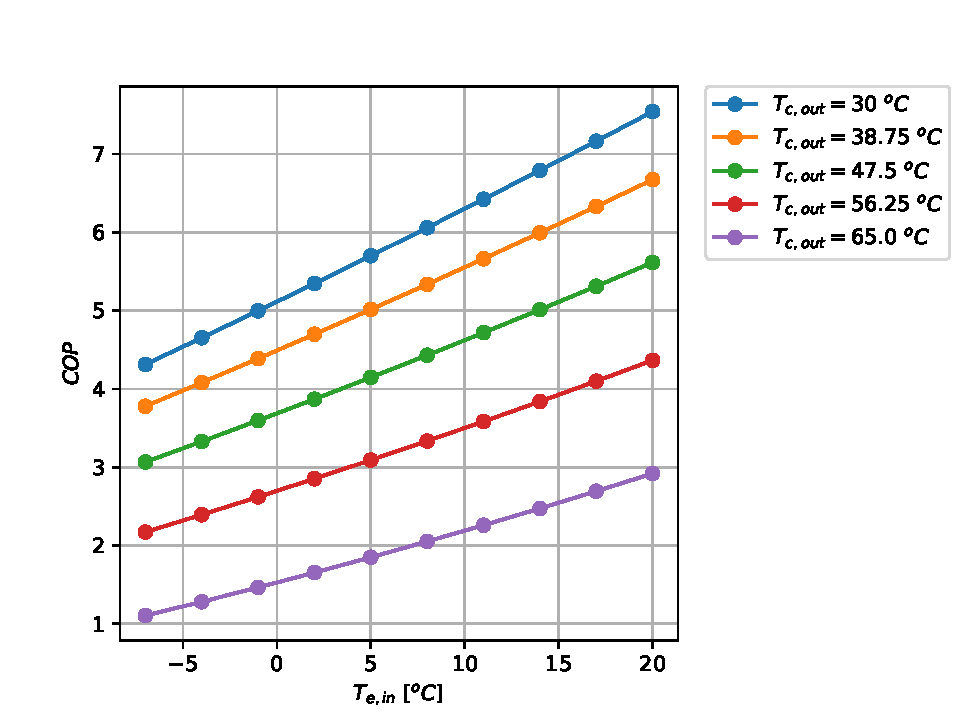
\includegraphics[width=1\textwidth]{C:/Daten/spfPackages/GIT/spfTrnsysFiles/HeatPump/BrineToWater/Walter Meier/SIN-75TU/SIN-75TU-Cop.pdf}
\caption{COP Results for the heat pump at the selected points}
\label{COPFig}
\end{center}
\end{figure}
\begin{figure}[!ht]
\begin{center}
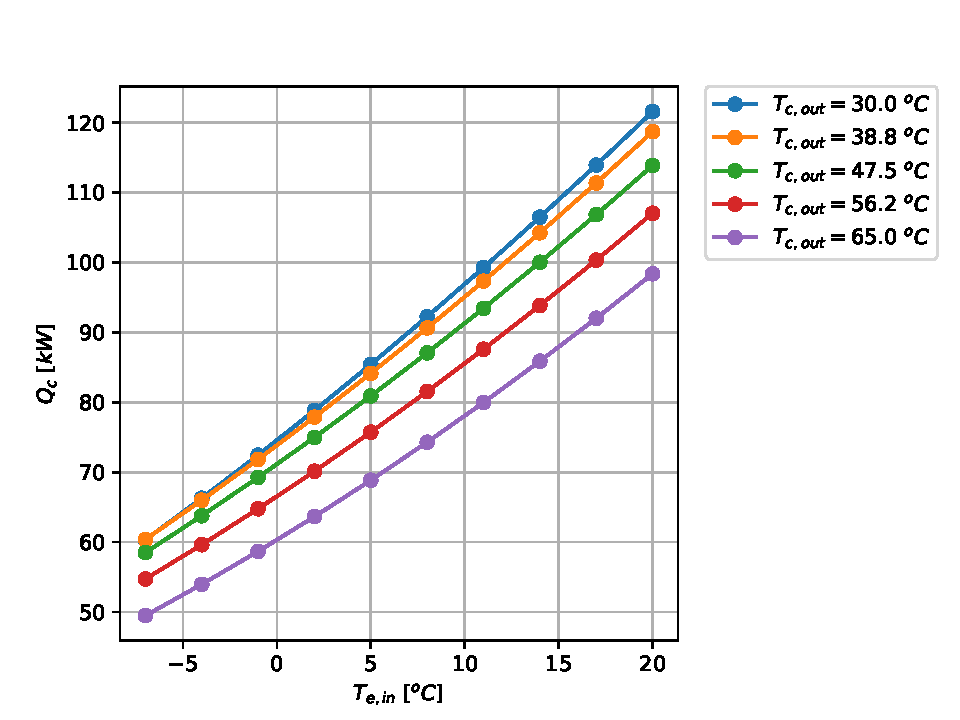
\includegraphics[width=1\textwidth]{C:/Daten/spfPackages/GIT/spfTrnsysFiles/HeatPump/BrineToWater/Walter Meier/SIN-75TU/SIN-75TU-Qc.pdf}
\caption{$Q_c$ Results for the heat pump at the selected points}
\label{QcFig}
\end{center}
\end{figure}
\end{document}
